\section{Interface}\label{sec:gui}

User interaction is accomplished through a simple Graphical User Interface, providing the most of the controls as sliders.
The upper area controls the LFO parameters. In figure~\ref{fig:gui-lfo} we can notice how the controls are always relevant to the selected waveform, i.e. for the ``random wave'' the ``phase'' slider is replaced with a ``width'' slider (see section~\ref{sec:parameters} for more details on LFO parameters).

\begin{figure}[H]
	\centering
	\subcaptionbox{Sinusoidal shape}{
		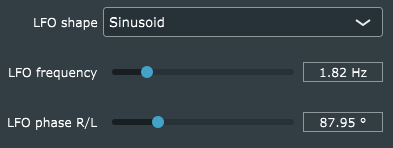
\includegraphics[width=0.5\linewidth]{assets/gui-lfo1.png}
	}%
	\subcaptionbox{Random shape}{
		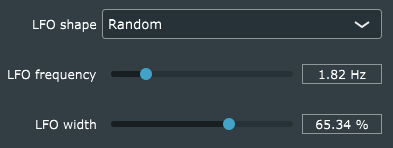
\includegraphics[width=0.5\linewidth]{assets/gui-lfo2.png}
	}
	\caption{Different parameters depending on the LFO shape}
	\label{fig:gui-lfo}
\end{figure}

The remaining controls affect the main effect parameters.

\begin{description}
	\item[Sweep width] controls the peak delay of the LFO;
	\item[Depth] controls the intensity of the effect, like a dry/wet control, and corresponds to the gain level of the delay line;
	\item[Feedback] controls the intensity of the feedback, corresponds to the gain of the feedback loop;
	\item[HP cut-off] controls the cut-off frequency of the high-pass filter;
	\item[Invert polarity] controls whether the wet signal is added or subtracted from the dry signal.
\end{description}

The full GUI as it is presented to the user is shown in figure~\ref{fig:gui-all}.

\begin{figure}
	\centering
	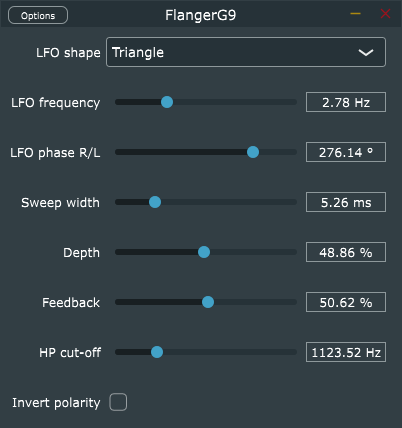
\includegraphics[width=0.5\linewidth]{assets/gui-all.png}
	\caption{Complete Graphical User Interface}
	\label{fig:gui-all}
\end{figure}

\subsection{Implementation Details}\label{sec:gui-implementation}

\nocite{juce}

In order to avoid code duplication, we adopted some techniques to define the GUI using a more descriptive approach rather than an imperative approach.

In particular, each \texttt{Slider} is dynamically generated in a \texttt{for} loop, which iterates over an array of \texttt{UISliders} objects describing the properties of each slider (i.e. label, unit, range and binding functions).
The initial \texttt{ComboBox} is populated by iterating over a \texttt{std::map} which associates each \texttt{OscFunction} enum value to the corresponding label. The final \texttt{ToggleButton}, being just one, is added directly.

Each \texttt{Component} is then added to an \texttt{Array}, which is iterated over during the \texttt{resized()} method, and laid down using a vertical main-axis \texttt{FlexBox}, to prevent hard-coding numerical values for bounds and sizes. For the styling we just kept JUCE's default \texttt{LookAndFeel}, being already clear enough for this purpose.

Value changes are bound using lambda-functions, instead of subclassing \texttt{Listener}, for easier coding.
In particular, the logic of alternating the display between the two ``phase'' and ``width'' \texttt{Slider}s is accomplished by keeping a map of ``mutually exclusive'' \texttt{Component}s. The correct \texttt{Slider} is then displayed when the \texttt{ComboBox.onChange} lambda-function is invoked.

Value unit conversion is finally performed by \texttt{FlangerProcessor}'s setter/getter methods of each parameter, following the encapsulation pattern to bridge between UI and internal representations.